\documentclass[aps,twocolumn,secnumarabic,nobalancelastpage,amsmath,amssymb,
nofootinbib,superscriptaddress]{revtex4-1}


\usepackage{graphics}       % standard graphics specifications
\usepackage{graphicx}       % alternative graphics specifications
\usepackage{longtable}      % helps with long table options
\usepackage{url}            % for on-line citations
\usepackage{bm}             % special 'bold-math' package
\usepackage[ngerman]{babel} % deutsche Siblentrennung
\usepackage[utf8]{inputenc} % Umlaute

\def\andname{\hspace*{-0.5em},} % definiert die Trennung zwischen 2 Autoren neu

% Titelseite
\begin{document}
\title{F-Praktikum: Elektrolumineszenz-Spektroskopie}
\author         {Ch. Egerland}
\email[Email: ]{egerlanc@physik.hu-berlin.de}
\author         {M. Pfeifer}
\email[Email: ]{mpfeifer@physik.hu-berlin.de}
\affiliation    {Humboldt-Universität zu Berlin, Institut für Physik}
\date[Versuchsdatum: ]{06.07.2017}

%%%%%%%%%%%%%%%%%%%%%%%%%%%%%%%%%%%%%%%%%%%%%%%%%%%%%%%%%%%%%%%%%%%%%%%%%%%%%%%%
\begin{abstract}
Untersucht wird das Lumineszenzspektrum einer InGaP/GaAs-Photodiode im Temperaturbereich zwischen
$80\text{ K}$ und $255\text{ K}$. Die Fluoreszenzmessung wird mithilfe eines Czerny-Turner-Spektrometers
und einer Photomultiplier-Tube realisiert. Wir treffen Aussagen über den Verlauf des Spektrums, die
Temperaturabhängigkeit des Lumineszenzpeaks, den thermischen Einluss auf die integrierte Peakintensität und
wir geben eine Abschätzung für die Aktivierungsenergie zur Lumineszenz von InGaP an.
\end{abstract}


\maketitle


%%%%%%%%%%%%%%%%%%%%%%%%%%%%%%%%%%%%%%%%%%%%%%%%%%%%%%%%%%%%%%%%%%%%%%%%%%%%%%%%

\section{Theorie}

\noindent Unter Lumineszenz versteht man Strahlung, die beim Übergang eines Systems von einem angeregten Zustand
in einen niederenergetischen Zustand emittiert wird. Bei Halbleitern lassen sich diese Übergänge mit dem Bändermodell
beschreiben. So finden die elektronischen Übergänge vor allem aus dem Leitungsband ins Valenzband statt, so dass bei
Anregung des Materials mit ausreichend Energie ($E>E_g$) Lumineszenzphotonen mit einer der Bandlücke entsprechenden
Frequenz erzeugt werden (direkter Übergang).\newline

\noindent Es gibt verschiedene Rekombinationswege für ein sich im angeregten Zustand befindlichendes System (s. Abb. \ref{fig:rekomb} ) \cite{saarland}.
Liegt ein dotierter Halbleiter vor, speziell z.B. eine Heterostruktur mit pn-Übergang, gibt es im Bereich zwischen Leitungs-
und Valenzband Donator- (knapp unter Leitungsbandkante) und Akzeptorzustände (knapp über der Valenzbandkante). Ebenfalls für die
Lumineszenz relevant sind sog. Exzitonen-Zustände (gebundene Elektron-Loch-Paare). Bei guter Kühlung (wenig thermischer
Anregung) sind neben dem direkten Übergang (LB$\rightarrow$VB) daher auch andere Übergänge, z.B. Exzitonen-Rekombination,
Übergänge vom Donator- zum Akzeptorniveau (D,A) oder ins Valenzband (D,h) sichtbar. Im Falle von InGaP lässt sich die exzitonische
Bindungsenergie mit den effektiven Elektron-/Lochmassen, gegeben in \cite{anleitung}, in der Wasserstoffnäherung berechnen:
\begin{eqnarray}
  E_{n} = \frac{\mu\cdot e^4}{32\pi^2\hbar^2\epsilon^2\epsilon_0^2}\cdot\frac{1}{n^2}
  \\[6pt]
  \nonumber
  E_{n}<E_{1} = 7\text{ meV}\;\;\;\;\,\,\,
  \label{eq:exitEbind}
\end{eqnarray}

\noindent Dabei bezeichnet $\mu=\left(\frac{1}{{m_e}^*} +\frac{1}{{m_h}^*}\right)^{-1}$ die reduzierte Masse des Exzitons.
Die Permittivität der InGaP/GaAs-Heterostruktur wurde als $\epsilon=11.75\epsilon_0$ angenommen \cite{dielek}.

\begin{figure}[h]
  \centering
  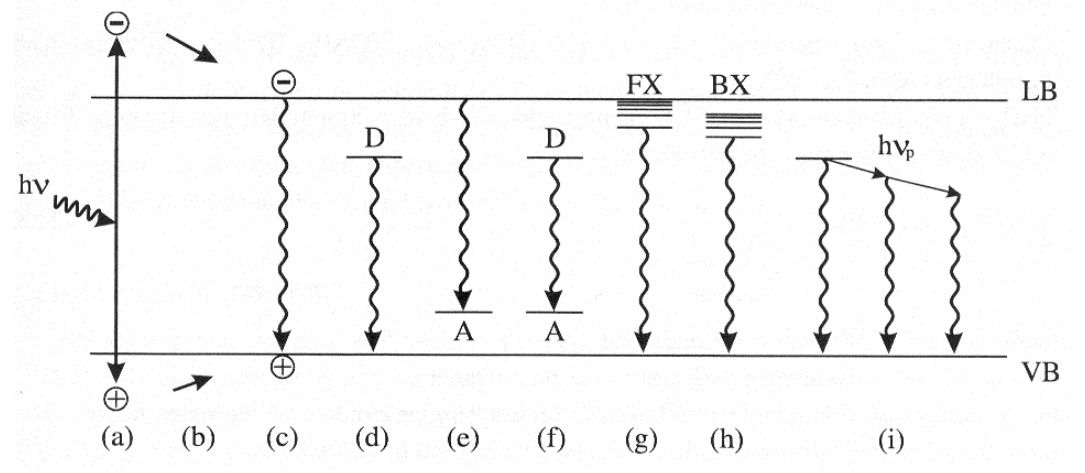
\includegraphics[width=0.47\textwidth]{img/rekombinationswege.jpg}
  \caption{ Lumineszenz-relevante elektronische Übergänge: a) Anregung, b) Relaxation im Band,
  c) (e,h)-Übergang, d) (D,h)-Übergang, e) (e,A)-Übergang, f) (D,A)-Übergang, g) Rekombination freier Exzitonen; aus: \cite{saarland}}
  \label{fig:rekomb}
\end{figure}


%%%%%%%%%%%%%%%%%%%%%%%%%%%%%%%%%%%%%%%%%%%%%%%%%%%%%%%%%%%%%%%%%%%%%%%%%%%%%%%%

\section{Experiment}

\noindent Der Versuchsaufbau ist schematisch in Abbildung \ref{fig:versuch} dargestellt. Die Anregung der Diode erfolgt durch Anlegen einer
Spannung mittels einer externen Versorgung, die einen konstanten Strom von $I=30\text{$\mu$A}$ liefert. Dazu sind die elektrischen Verbindungen bereits an der Probe angebracht.
Diese befindet sich in einem evakuierten ($p\sim 2\text{ Pa}$) und auf $80\text{ K}$ Stickstoff-temperierten Kryostaten. Die Temperaturmessung
erfolgt durch einen Sensor, der möglichst nahe an der Probe platziert wurde.

\begin{figure}[h]
  \centering
  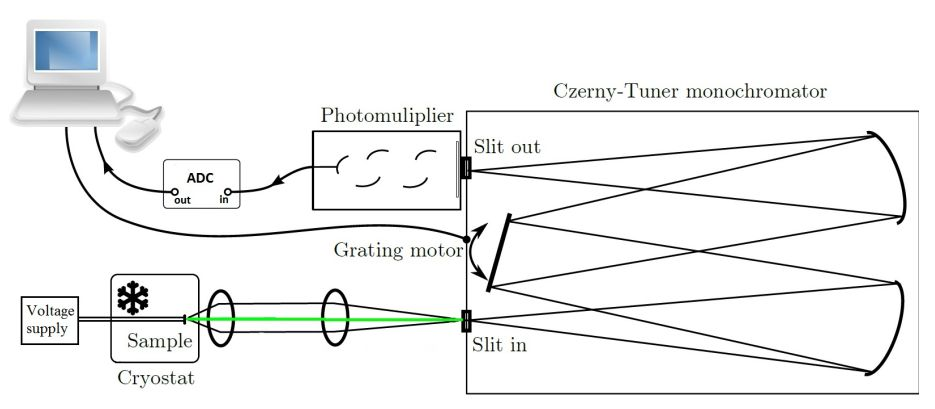
\includegraphics[width=0.48\textwidth]{img/versuchsanleitung.jpg}
  \caption{Versuchsaufbau, aus: \cite{anleitung}}
  \label{fig:versuch}
\end{figure}

\noindent Die durch Rekombination entstandenen Photonen gelangen zunächst durch eine Kollimatorlinse, gefolgt von einer Linse zur
Strahlfokussierung und treffen dann auf ein Czerny-Turner-Monochromator. Durch die Beweglichkeit des Gitters im
Monochromator (Schrittmotorsteuerung) können verschiedene Spektralbereiche selektiert werden, deren Intensität anschließend in einem Photomultiplier (PMT)
gemessen wird. Dieser arbeitet mit einer Beschleunigungsspannung von $U_\text{PMT}=2,2\text{ kV}$. Zwecks Maximierung des
Signal-Rausch-Verhältnisses wurde die PMT ebenfalls gekühlt (Peltierelement mit Wasserkühlung). Das Signal der Photonenvervielfachers
gelangt dann über einen Analog-Digital-Wandler zum Computer, der die Messsignale zusammen mit der Schrittmotorposition des Monochromators
abspeichert und zu einem Energiespektrum verarbeitet.


%%%%%%%%%%%%%%%%%%%%%%%%%%%%%%%%%%%%%%%%%%%%%%%%%%%%%%%%%%%%%%%%%%%%%%%%%%%%%%%%

\section{Daten und Analyse}
\subsection{Vorüberlegungen}

\noindent Um eine bessere Einordnung der Ergebnisse zu ermöglichen, wird zunächst mithilfe einer empirischen
Formel die temperaturabhängige Lage des Lumineszenzpeaks (entspricht Größe der Bandlücke) geschätzt.
Hierzu berechnen wir zunächst in welcher Zusammensetzung $\text{Ga}_x\text{In}_{1-x}\text{P}$
an GaAs gitterangepasst ist durch: $a_{GaAs} = x\cdot a_{GaP}+(1-x)\cdot a_{InP}$. Wir finden
$x=0,515$ und mit der empirischen Formel (bei $\text{T}=300\text{ K}$) \cite{vorbereitung}:
\begin{equation}
  E_{g}(x) = 1,351+0,643x+0,786x^2\text{ (eV) }
   \label{eq:Ex}
\end{equation}

\noindent eine geschätzte Bandlückenenergie mit entsprechender Wellenlänge von
\begin{equation}
  E_g \approx 1.89\text{ eV} \Rightarrow  \lambda \approx 656,52\text{ nm}
  \label{eq:evEgap300K}
\end{equation}

\noindent Um nun die Verschiebung von $E_g$ mit der Temperatur zu bestimmen, wurden
die temperaturabhängigen Bandlückenenergien von InP und GaP gewichtet und wir erhalten
die orangene Kurve in Abb. \ref{fig:EgapT} mit einer Differenz zwischen $T=80\text{ K}$
und $T=300\text{ K}$ von:

\begin{equation}
  \Delta E_g \approx 60\text{ meV} \Rightarrow \Delta\lambda \approx 20.0\text{ nm}
\label{eq:evVersch}
\end{equation}

%%%%%%%%%%%%%%%%%%%%%%%%%%%%%%%%%%%%%%%%%%%%%%%%%%%%%%%%%%%%%%%%%%%%%%%%%%%%%%%%
\subsection{Analyse der Spektren}

\noindent Die bei verschiedenen Temperaturen aufgenommenen Spektren sind in Abbildung \ref{fig:spek} dargestellt.
Deutlich zu erkennen ist die Abnahme der Lumineszenzintensität und die Peakverbreiterung bei steigenden Temperaturen.
Oberhalb von ca. $165\text{ K}$ ist ein Verschmieren der linken Peakhälften hin zu kürzeren Wellenlängen zu erkennen.
Deshalb und da bereits ab $T>100$ K ein asymmetrischer Verlauf der Kurven zu erkennen ist, wurden alle Lumineszenzpeaks
einem Doppelgaußfit unterzogen (Mathematica).
Exzitonische Übergänge konnten nicht beobachtet werden. Dies lässt sich leicht
einsehen, wenn man die mittlere kinetische Energie eines Teilchens mit $k_B T\approx 7\text{ meV}$ bei $T=80$ K nähert und
mit der exzitonischen Bindungsenergie (\ref{eq:exitEbind}) vergleicht. Offensichtlich ist die Temperatur
von 80 K zu hoch, um exzitonische Übergänge zu beobachten, da gerade genügend thermische Energie zur Verfügung steht
um die exzitonische Bindungsenergie zu überwinden.

Entscheidend für die Temperaturabhängigkeit der Lumineszenz ist die bei steigenden Temperaturen immer
relevantere Elektron-Phonon-Wechselwirkung. Vernachlässigbar bei geringen Temperaturen sorgen diese Wechselwirkungen
bei großen Temperaturen für die sichtbare Verbreiterung der Peaks (Impulsübertrag von $e^-$ auf Phonon und umgekehrt führt
zu geringfügig niedrigeren/höheren Photonenenergien) \cite{phonons}.

\begin{figure}[t]
  \centering
  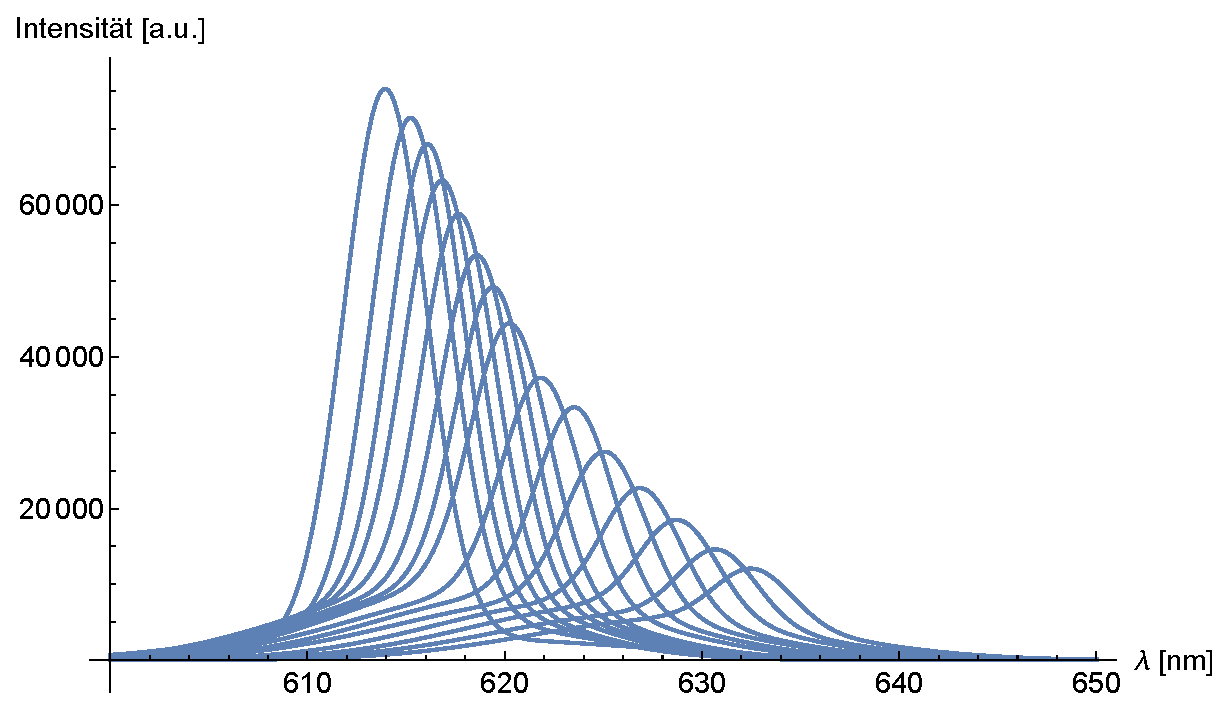
\includegraphics[width=0.48\textwidth]{../Messung/allfitsplot.eps}
  \caption{\label{fig:spek} (1,2-fach) gauß-gefittete Lumineszenzspektren von InGaP zwischen $80\text{ K}$ und $250\text{ K}$ (vlnr)}
\end{figure}

%%%%%%%%%%%%%%%%%%%%%%%%%%%%%%%%%%%%%%%%%%%%%%%%%%%%%%%%%%%%%%%%%%%%%%%%%%%%%%%%
\subsection{Temperaturabhängigkeit der Bandlückenenergie}

\noindent Die Erwärmung des Kristalls führt zu einer Verschiebung der Valenz- und Leitungsbänder und insbesondere
zu einer Verkleinerung der Bandlücke, die gemäß der Varshni-Formel abgeschätzt werden kann:
\begin{equation}
  E_g(T) = E_g(\text{T}=0\text{ K})-\alpha\cdot\frac{T^2}{T+\beta}
   \label{eq:varshni}
\end{equation}

\noindent In den Abbildungen \ref{fig:EgapT} \& \ref{fig:lamT} sind die Temperatur-
abhängigkeiten der Bandlückenenergie und der entsprechenden Wellenlänge dargestellt. Bei steigenden Temperaturen wurde eine deutliche
Rotverschiebung des Intensitätsmaximums gemessen (Verkleinerung der Bandlücke). Die Rotverschiebung konnte auch durch
direkte Beobachtung festgestellt werden. Grund hierfür ist neben der thermischen Ausdehnung des Kristallgitters (Verringerung
der Bindungsenergie der Gitterelektronen/-löcher) die Veränderung des effektiven Kristallpotentials durch bei höheren Temperaturen
zunehmende Elektron-Phonon-Streuung \cite{kittel}.

Führt man eine Extrapolation der experimentellen Daten (Bandlücke/Wellenlänge zwischen 80 K und 255 K) durch und
betrachtet die erwarteten Verschiebungen im Bereich zwischen 80 K und 300 K, lassen sich die Ergebnisse mit (\ref{eq:evVersch})
vergleichen:
\begin{equation}
  \Delta E_{g,exp}\approx 74\text{ meV} \Rightarrow \Delta\lambda_{exp}\approx 23.5\text{ nm}
   \label{eq:expVersch}
\end{equation}

\begin{figure}[t]
  \centering
  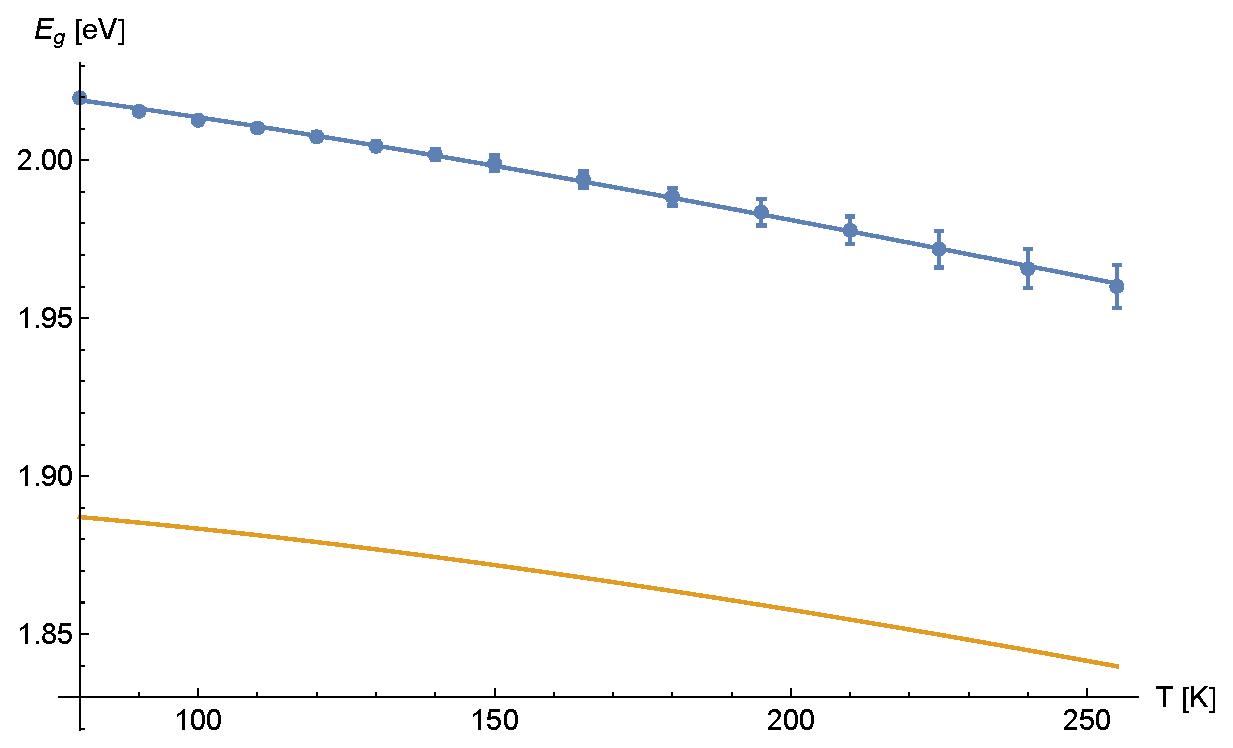
\includegraphics[width=0.48\textwidth]{../Messung/energtemp.eps}
  \caption{\label{fig:EgapT} Bandlückenenergie in Abhängigkeit der Temperatur, Fitparameter
  aus Varshniformel: $E_g^0= 2.03 \text{ eV}$, $\alpha = 4.3*10^{-4}\text{ eV/K}$, $\beta = 140.2 \text{ K}$}
\end{figure}

\noindent Die Größenordnung und Richtung der Wellenlängenverschiebung deckt sich mit der Erwartung aus (\ref{eq:evVersch}).
Die gemessene Änderung der Bandlücke - wie auch die Wellenlängenänderung - ist jedoch etwas größer ausgefallen als die Theorie vorhersagt.
Diese Diskrepanz könnte sowohl von Verunreinigungen des Kristalls als auch von einer abweichenden Materialzusammensetzung als oben angenommen
herrühren. Die konkrete Abweichung der experimentell ermittelten Bandlücke von der Theoretischen gibt Aufschluss über die Mengenverhältnisse von
Ga und In in der Diode. Die Materialzusammensetzung war vermutlich nicht genau gitterangepasst an GaAs, da die erhaltene
Bandlücke experimentell größer ausgefallen ist als theoretisch vorhergesagt (s. Abb. \ref{fig:EgapT}). Neben Verunreinigungen des Materials könnte
die Ursache hierfür gemäß \ref{eq:Ex} ein höherer Gehalt an Ga (GaP) sein (d.h. $x>0.51$).
Extrapoliert man die experimentell ermittelte Bandlücke für $T=300\text{ K}$ mithilfe der Varshni-Formel, lässt sich mit Gl. (\ref{eq:Ex})
ein korrigierter Wert für die Zusammensetzung errechnen. Wir erhalten $x_{korr}\approx 0.55$.

\begin{figure}[h]
  \centering
  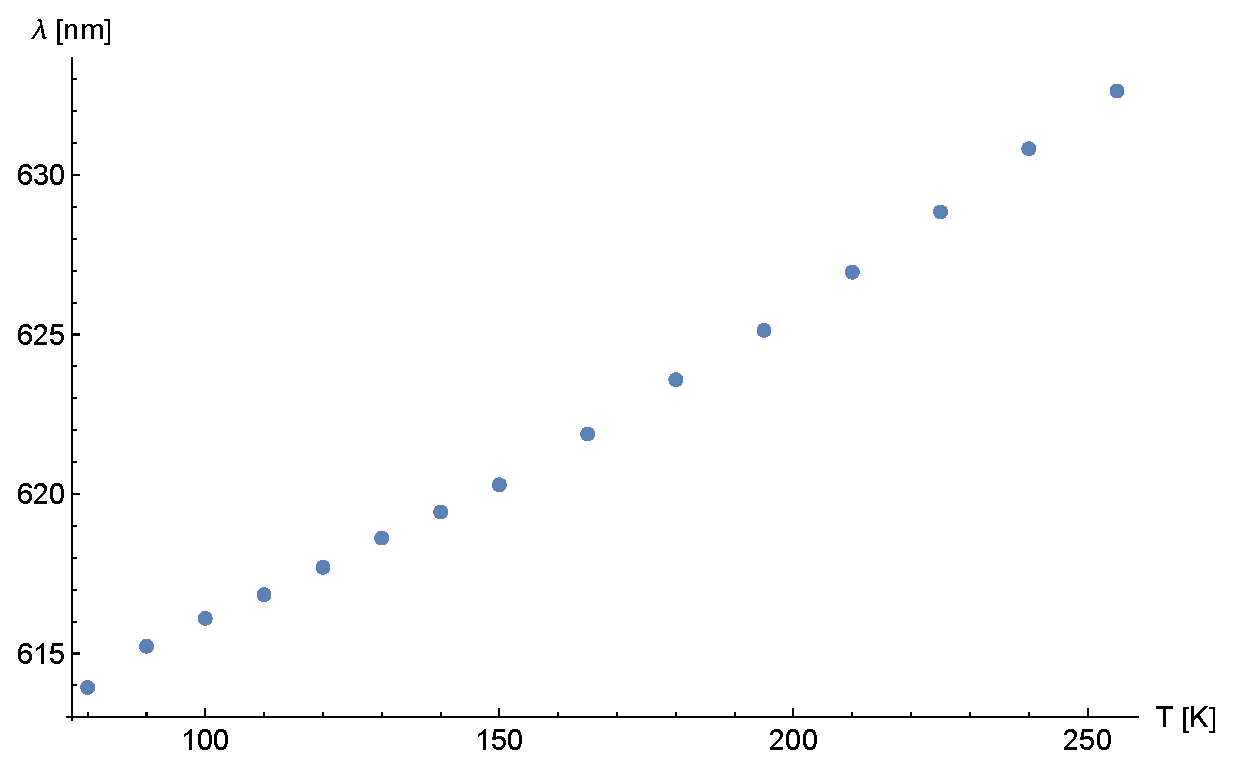
\includegraphics[width=0.48\textwidth]{../Messung/peaktemp.eps}
  \caption{\label{fig:lamT} Temperaturabhängigkeit der Lumineszenz-Wellenlänge von InGaP}
\end{figure}

%%%%%%%%%%%%%%%%%%%%%%%%%%%%%%%%%%%%%%%%%%%%%%%%%%%%%%%%%%%%%%%%%%%%%%%%%%%%%%%%
\subsection{Temperaturabhängigkeit der Intensitäten}

\begin{figure}[b]
  \centering
  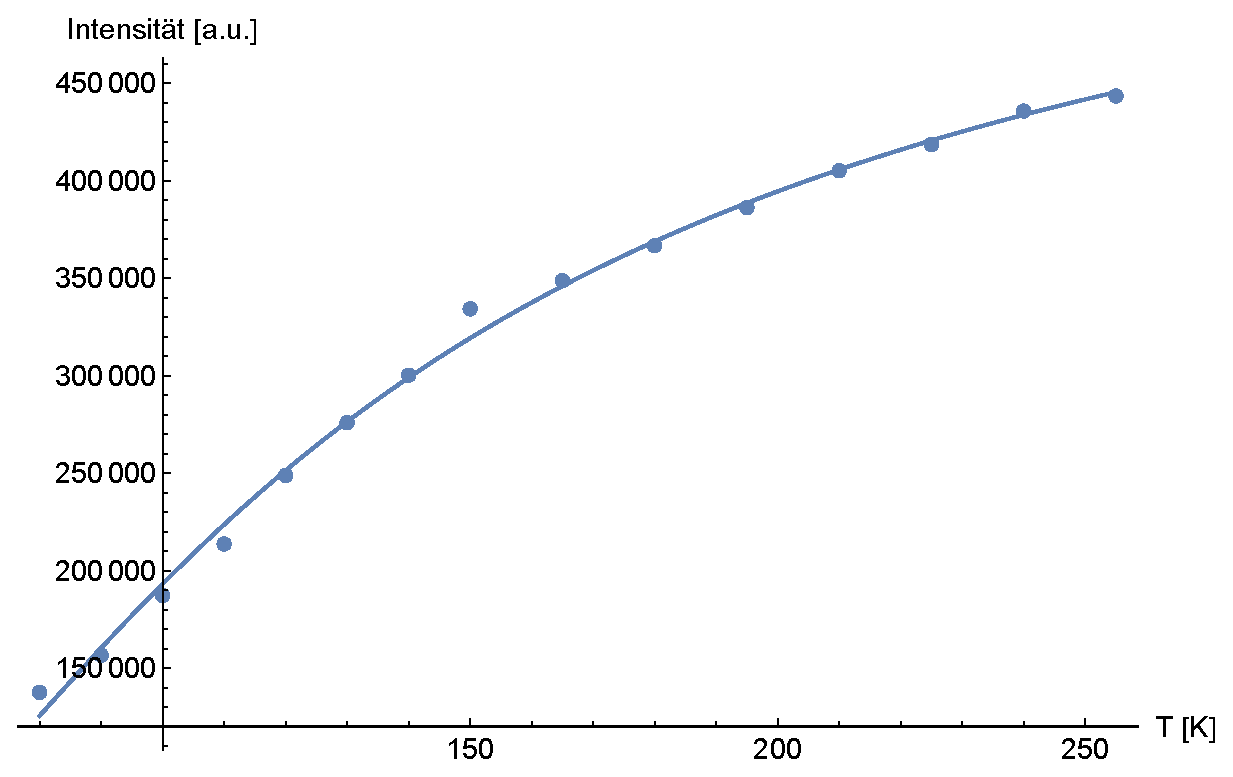
\includegraphics[width=0.48\textwidth]{../Messung/integrintenstempfit.eps}
  \caption{\label{fig:intInt}Integrierte Intensitäten der Lumineszenzpeaks in Abhängigkeit
  der Temperatur,
  Fitparameter aus Arrheniusgleichung: $I_0=450074$, $c=25.2$, $E_A=33.4\text{ meV}$}
\end{figure}

\noindent Die Abnahme der Lumineszenzintensität bei steigenden Temperaturen lässt sich mit der Fermi-Dirac-Verteilung
verstehen: bei steigenden Temperaturen werden zunehmend auch Zustände oberhalb der Fermi-Energie, also Zustände
im Leitungsband bzw. Donatorzustände besetzt, die aufgrund ausreichend thermischer Energie nicht ins Valenzband
rekombinieren und somit für eine Verminderung der Anzahl der abgestrahlten Photonen pro Zeit (und Fläche) sorgen.
Außerdem können aufgrund von Elektron-Phonon-Wechselwirkungen (insb. bei hohen Temperaturen) mehr Ladungsträger durch
Schwingungsrelaxation, also nicht-strahlend, ins Valenzband rekombinieren, was ebenfalls zu einer Reduktion des
Photonenflusses führt.

Die integrierten Intensitäten der Spektrallinien sind in Abb. \ref{fig:intInt} dargestellt. Erkennbar ist
die Abnahme der Peak-Flächen bei steigenden Temperaturen. Mit Hilfe der Arrheniusgleichung lassen sich die integrierten
Peakintensitäten in Abhängigkeit von der Temperatur fitten und somit Rückschlüsse auf die Aktivierungsenergie $E_A$ ziehen.

  \begin{equation}
    I(T) = \frac{I_0}{1+c\cdot\text{exp}\left( -\frac{E_A}{k_B T} \right)}
  \end{equation}

\noindent Diese beschreibt die notwendige Energie eines Ladungsträgers im Donator-/Akzeptorniveau, um ins nächstgelegene Band
(Leitungs-/Valenzband) angeregt zu werden, um dann strahlend, über Phononen oder andere nicht-strahlende Prozesse zu relaxieren.
In Abb. \ref{fig:intInt} ist dieser Fit dargestellt. Wir erhalten eine Aktivierungsenergie von $E_A=33 \text{ meV}$, welche im erwarteten
Referenzbereich von $E_A=(10-50)\text{ meV}$ (für Ga$_{0.52}$In$_{0,48}$P) \cite{eact} liegt.

In Abb. \ref{fig:maxInt} sind die maximalen Intensitäten über die Temperatur aufgetragen. Deutlich ist wieder
der (stärker als lineare) Abfall der Lumineszenz-Intensität bei steigenden Temperaturen. Wie bereits in Abschnitt III.2 erläutert,
sind vor allem Elektron-Phonon-Wechselwirkungen für dieses Verhalten verantwortlich.

\begin{figure}[t]
  \centering
  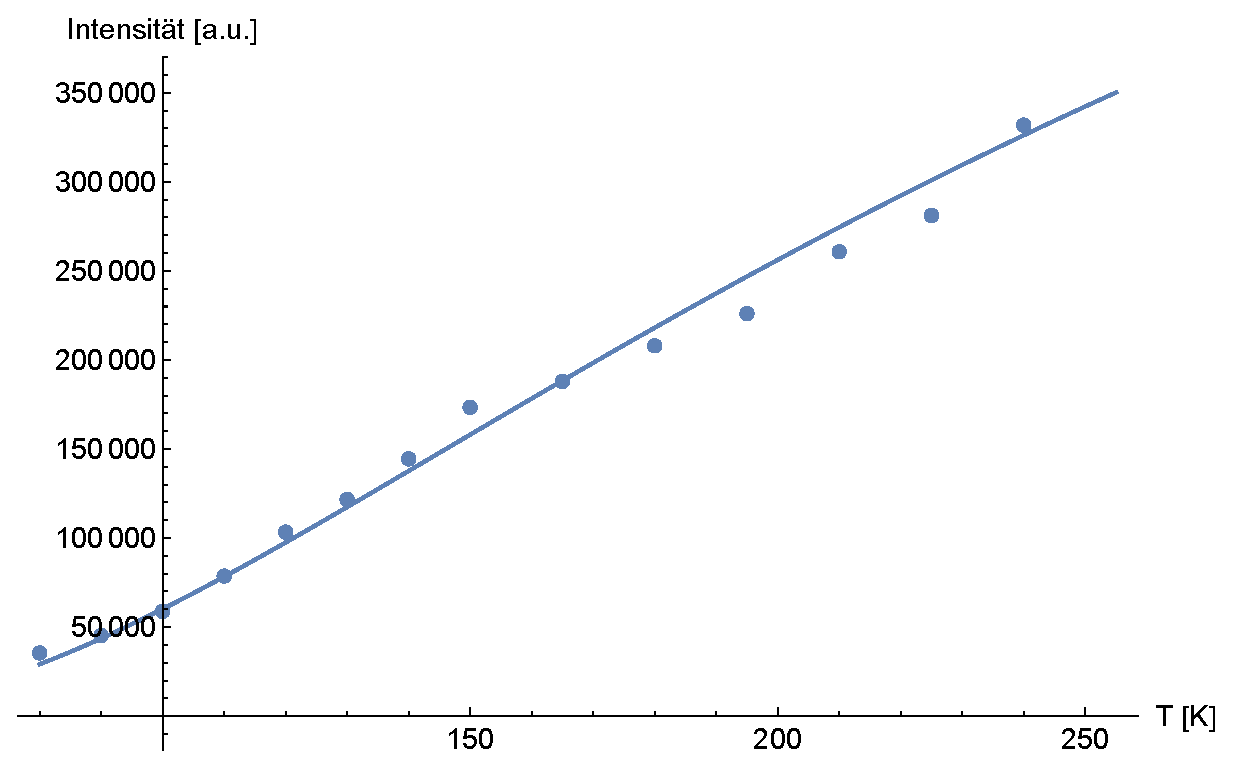
\includegraphics[width=0.48\textwidth]{../Messung/maxintenstempfit.eps}
  \caption{\label{fig:maxInt}Maximale Intensität der Lumineszenzpeaks bei $T=80\text{ K}$ bis $T=250\text{ K}$ (vlnr)}
\end{figure}

%%%%%%%%%%%%%%%%%%%%%%%%%%%%%%%%%%%%%%%%%%%%%%%%%%%%%%%%%%%%%%%%%%%%%%%%%%%%%%%%
\section{Schlussfolgerung}

\noindent Es wurde das Lumineszenzspektrum einer InGaP/GaAs-Photodiode untersucht. Die charakteristische Temperaturabhängigkeit der
Bandlücke, sowie der Peakintensitäten und integrierten Peakintensitäten konnte bestätigt werden. Mittels Vergleich des theoretischen
und experimentellen Temperaturverhaltens der Bandlücke wurde eine Aussage über die Zusammensetzung des Ga$_x$In$_{1-x}$P getroffen
($x>0.51$). Die auf die Lumineszenz bezogene ermittelte Aktivierungsenergie von InGaP liegt im erwarteten Bereich.
Unreinheiten in der Kristallstruktur wurden während der gesamten Betrachtung quantitativ vernachlässigt. Diese würden zur Bildung
von Zwischenniveaus in der Bandlücke führen. Die Absorptionskante würde dadurch, je nach Dotierung, nach oben oder unten verschoben werden, was
zu einer systematischen Abweichung der Bandlücke führen würde.

%%%%%%%%%%%%%%%%%%%%%%%%%%%%%%%%%%%%%%%%%%%%%%%%%%%%%%%%%%%%%%%%%%%%%%%%%%%%%%%%
\bibliography{sample-paper}
\bibliographystyle{prsty}
\begin{thebibliography}{99}
\bibitem{saarland}Prof. Dr. Thomas Wichert, Photolumineszenz-Spektroskopie an Halbleitern, Universität des Saarlandes [2006]
\bibitem{anleitung}FET Group, Benutzerhandbuch Elektrolumineszenz-Spektroskopie, Humboldt-Universität zu Berlin
\bibitem{vorbereitung}FET Group, Fragen zur Vorbereitung, S.1-3, Humboldt-Universität zu Berlin
\bibitem{kittel}Ch. Kittel, Einführung in die Festkörperphysik, S.159f., 12. Auflage, Oldenbourg Verlag [1999]
\bibitem{phonons}C. Besikci and M. Razeghi, Electron Transport Properties of Ga$_{0.51}$In$_{0.49}$P for Device Applications, IEEE Trans.Electron Devices, vol. 41, no. 6, pp. 1066-1069 [1994]
\bibitem{dielek}S. Adachi, Material Parameters of In$_{1-x}$Ga$_x$As$_y$P$_{1-y}$ and Related Binaries, J.Appl.Phys., vol. 53, no. 12, pp. 8775-8792 [1982]
\bibitem{max}Woo Sik Yooa, Kitaek Kanga, Gota Muraib and Masahiro Yoshimotob, Temperature Dependence of Photoluminescence Spectra from Crystalline Silicon, Kyoto Institute of Technology [2015]
\bibitem{eact}J. D. Lambkin, L. Considine, and S. Walsh, Temperature dependence of the photoluminescence intensity of ordered and disordered In$_{0,48}$Ga$_{0.52}$P, Appl. Phys. Lett. 65, 73 [1994]
\end{thebibliography}


%%%%%%%%%%%%%%%%%%%%%%%%%%%%%%%%%%%%%%%%%%%%%%%%%%%%%%%%%%%%%%%%%%%%%%%%%%%%%%%%
\clearpage
\appendix
%%%%%%%%%%%%%%%%%%%%%%%%%%%%%%%%%%%%%%%%%%%%%%%%%%%%%%%%%%%%%%%%%%%%%%%%%%%%%%%%


\end{document}
